\graphicspath{{capitulos/Capitulo6-Conclusiones/recursos/}}


\section{Conclusiones} \label{capitulo:6}

El problema que tenemos entre manos, que se ha descrito en profundidad en el \autoref{capitulo:2}, trata de automatizar el proceso de conformar una planificación de asignación de trabajo de los controladores aéreos de un puesto de control concreto en caso de que suceda una incidencia que puede ser de dos tipos: cambio de la sectorización esperada (predicha con antelación) o bien una baja de uno de los controladores, con una posible alta de otro.

%lea dos fases diferentes: la \faseuno{} emplea diferentes heurísticas de inicialización de la solución inicial para la \fasedos{}, que trata de resolver el problema empleando la metaheurística \vns{} (VNS), de la que esperábamos mejores resultados que con el \sa{} (SA).


Se ha propuesto una metodología, detallada en el \autoref{capitulo:3}, desglosada en dos fases, una de inicialización, que emplea diferentes heurísticas de para poder adaptar la planificación de entrada a las nuevas exigencias originadas por las contingencias a tratar de resolver; y otra de resolución, donde empleamos la metaheurística implementada, \vns{} (VNS),  y adaptada al problema para obtener soluciones codificadas de forma matricial y cuya calidad es cuantificable mediante una función de evaluación, o fitness, que permite tanto a la metaheurística en sí como a nosotros mismos realizar comparaciones entre soluciones y diferentes ejecuciones. 

Empleando este indicador, entre otros, se ha procedido a realizar un ajuste de los parámetros previamente descritos del sistema, realizando un pequeño estudio del comportamiento de los mismos en función de los diferentes casos y valores. Por lo tanto, podemos decir que la hipótesis inicial \ref{H1} ha sido correcta: el problema ha sido resuelto exitosamente en el plazo acordado.

Además, de todos los diferentes tipos de VNS implementados, hemos concluido que aceptar soluciones peores no da soluciones buenas, funcionando mejor la versión \textit{Basic} o la \textit{Descendant} en todos los casos. En cuanto a la naturaleza de los entornos, hemos comprobado que para esta metaheurística con los entornos definidos aplicados a este problema, la toma de entornos según probabilidades no aporta lo suficiente en casi ningún caso de prueba.

También se ha realizado un estudio comparativo del sistema alterando únicamente la metaheurística empleada para poder evaluar la hipótesis inicial \ref{H2}. En vista de los resultados, podemos concluir que también es correcta, pues el VNS muestra resultados significativamente mejores que los obtenidos mediante el \sa{} (SA) y en algunas de las instancias de prueba empleadas el comportamiento del VNS es considerablemente mejor, en especial con relación a la primera de las funciones objetivo, \ref{O1}, catalogada como la más importante.

Por último, la hipótesis \ref{H3} hacía referencia a la eficiencia del sistema, y para evaluarla se ha realizado un estudio del rendimiento de este, del que se concluye que la eficiencia ha mejorado para la parte más ardua: el cómputo de la función de evaluación. Dicha mejoría se ha realizado mediante un uso mayor de la memoria dinámica del programa, almacenando temporalmente los resultados de la función fitness de cada solución en una estructura de datos de lectura rápida (de baja complejidad computacional). A su vez, también se han cambiado otras estructuras de datos de tipo listas por otras de menor complejidad computacional de lectura. Sin embargo, por falta de tiempo e importancia de esta hipótesis frente a todas las demás, no se ha realizado la mejoría que posiblemente sea más significativa: cambiar la representación de los turnos de trabajo por otra mejor que la actual, que emplea cadenas de texto, pues su acceso y modificación es computacionalmente más costoso que otras estructuras propuestas, y dichas acciones se repiten de forma continuada a lo largo de toda la ejecución.

\subsection{Líneas futuras de trabajo}
\label{sec:6:trabajo-futuro}

El proyecto entre manos es de un tamaño mayor que este TFM en sí, pues forma parte de una línea de investigación de \gls{CRIDA} para automatizar el proceso de asignación de trabajo a sus empleados. Dicho proyecto tiene sus orígenes en la planificación de las asigaciones de los controladores aéreos unos días antes de ponerla en uso, y por esta razón el tiempo del sistema no era un aspecto crucial. En dicha línea diferentes alumnos de máster y doctorado (citados a lo largo de este documento) realizaron sus trabajos en torno a ese problema. Una nueva línea de trabajo estudia la posibilidad de replanificar las asignaciones en el propio día de su uso, debido a ciertas contingencias habidas que no correspondan con la planificada con anterioridad, y donde el tiempo sí es significativo, el sistema debe ser lo más rápido posible.
%
%En este TFM se continúa la línea de trabajo mediante la inclusión de nuevas funcionalidades que se esperan en el sistema automatizado final: el manejo de ciertas contingencias descritas.

Una vez concluido este TFM, la línea de trabajo continuará para poder mejorar los resultados alcanzados para que puedan ser realmente empleados por el personal del Centro de Control. Dicha mejoría puede realizarse en diferentes líneas de trabajo que proponemos a continuación.

En primera instancia, podemos mejorar la definición de la \faseuno{}, empleando una heurística de inicialización diferente. Proponemos el uso de más de un tipo de plantillas, pues hasta ahora tan solo se ha utilizado las de tipo $3\times1$, cuando existen otras que permiten emplear menos controladores para un mayor número de sectores. 

Por ejemplo, en el caso de tener que añadir 3 nuevos sectores a la planificación inicial debido a que no se han podido sustituir por otros afines que se cierran, podemos emplear una plantilla $8\times3$, que es de la forma de la \autoref{fig:6:plantilla8x3}, donde cada letra representa un sector (mayúsculas en puesto ejecutivo, minúsculas en planificador) y un guion un periodo de descanso. Esta plantilla permite emplear un controlador menos de los que empleamos con las plantillas $3\times1$ (véase la \autoref{fig:3:plantilla-3x1}), pues añade 3 controladores para cada sector, una totalidad de 9 controladores. Otras posibles plantillas son la $4\times1$, que al tener más descansos permite más movilidad de periodos de trabajo de cara a la \fasedos{}. 

\begin{figure}
	\centering
	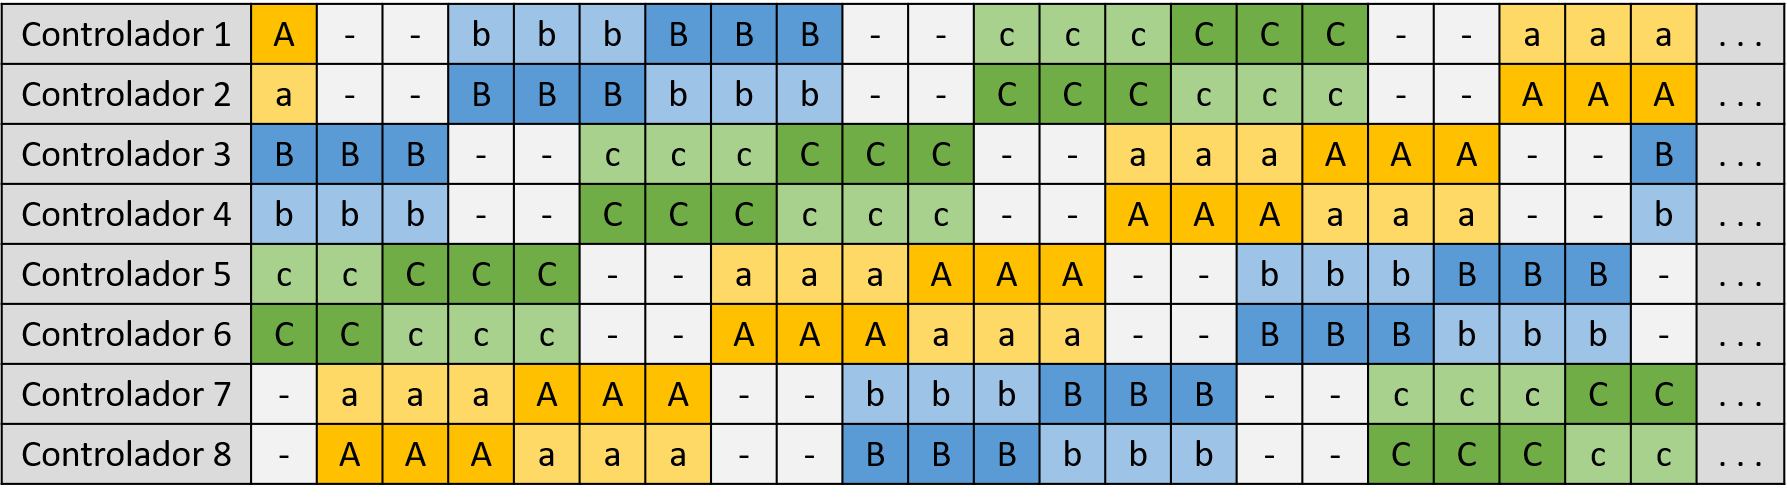
\includegraphics[width=\linewidth]{plantilla8x3}
	\caption{Aspecto de una plantilla $8\times3$.}
	\label{fig:6:plantilla8x3}
\end{figure}

En la definición de esta fase, la \autoref{sec:3:inicializacion-soluciones}, propusimos la implementación de un quinto paso para mejorar la calidad de la solución inicial. 
Además, se puede mejorar la eficiencia de la heurística de selección de sectores afines para su sustitución empleando un algoritmo más inteligente que simplemente uno de tipo voraz.

En segunda instancia, podemos mejorar la eficiencia de la \fasedos{}. Para ello se podrán emplear otras definiciones de entornos diferentes, y puesto que son la componente más relevante dentro de la metaheurística VNS, cambiarán notablemente el rendimiento de la misma. 

Otra línea por estudiar es el uso de otras funciones de distancia para el SVNS. Como hemos visto, en nuestra definición de SVNS y funciones de distancia no ha habido buenos resultados, pero esto no quiere decir que empleando otras funciones alternativas no se obtengan mejores resultados. 

Otra posibilidad para mejorar la eficiencia de la segunda fase consiste en emplear otra metaheurística diferente a VNS o SA, por ejemplo \textit{Tabu Search} (TS) (Búsqueda Tabú) o incluso otras técnicas de inteligencia artificial nombradas al inicio de la \autoref{sec:3:metaheurística} como \textit{Machine Learning} e incluso combinando diferentes técnicas.

Por otro lado, las soluciones alcanzadas por el sistema podrían aportar más valor a los expertos de CRIDA si se realizase un estudio en mayor profundidad de las necesidades de negocio de cara a ponderar de forma más precisa y personalizada las diferentes funciones objetivo, en lugar de utilizar el método ROC.

En tercera instancia, mejorar la eficiencia general del sistema, de la forma mencionada en la sección anterior: rediseñando las estructuras de datos básicas de representación de soluciones del sistema en su conjunto, lo que creemos aportará una mejora de eficiencia significativa. Otra opción es portar el sistema a otro lenguaje de programación más orientado a la eficiencia como puede ser C/C++. 

Por último, parece importante probar el sistema en más profundidad, pues los casos aportados por CRIDA para este trabajo no prueban todas las restricciones y casuísticas del problema entre manos. Un ejemplo de aspecto del dominio del problema que no ha sido probado son los sectores nocturnos. También sería adecuado realizar un estudio de casos de uso del sistema, que permita poder organizar y crear diferentes los casos de prueba de forma que se garantice que se prueban todas las funcionalidades requeridas por CRIDA.
